\section{Appendix}
\subsection*{Trace Plots}
In this section, we analyze the trace plots for the different models implemented. The analysis is consistent across all models due to the similarity of the trace plots. Notably, none of the trace plots display any distinct patterns. Furthermore, they appear to thoroughly explore the entire parameter space, as indicated by frequent transitions into various regions. The following plots were generated using a single chain; however, we have confirmed that the behavior remains consistent when using multiple chains.
\begin{figure}[H]
    \centering
    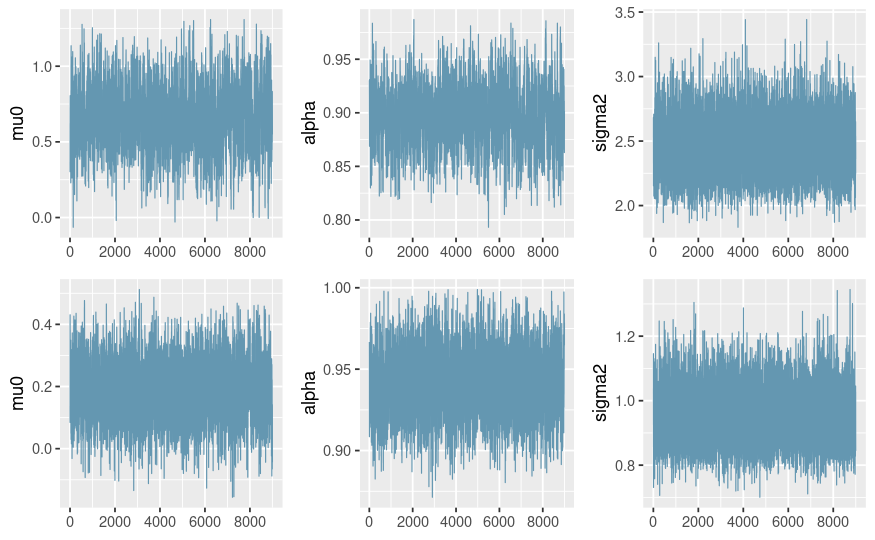
\includegraphics[width=0.9\textwidth]{images/2-AR/traceplots.png}
    \caption{Trace plots for the AR(1) models. The top line corresponds to the model used for GDP, while the bottom line corresponds to the model used for CPIAUCSL.}
\end{figure}
\begin{figure}[H]
    \centering
    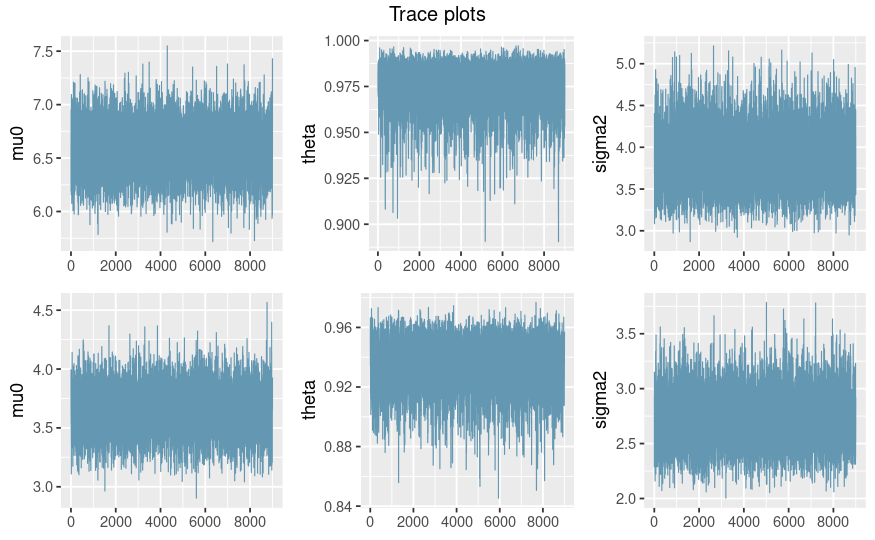
\includegraphics[width=0.9\textwidth]{images/3-MA/traceplots.png}
    \caption{Trace plots for the MA(1) models. The top line corresponds to the model used for GDP, while the bottom line corresponds to the model used for CPIAUCSL.}
\end{figure}
\begin{figure}[H]
    \centering
    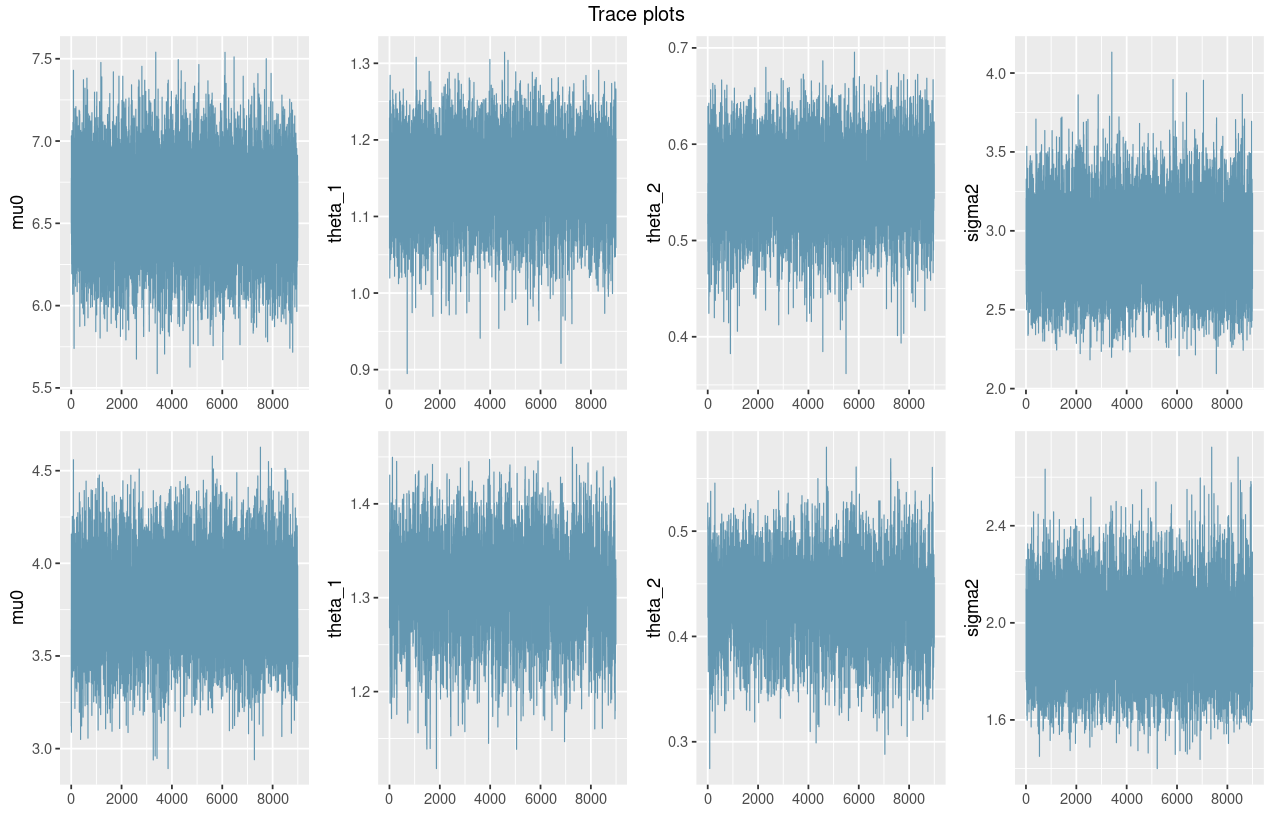
\includegraphics[width=0.9\textwidth]{images/3-MA/traceplots2.png}
    \caption{Trace plots for the MA(2) models. The top line corresponds to the model used for GDP, while the bottom line corresponds to the model used for CPIAUCSL.}
\end{figure}
\begin{figure}[H]
    \centering
    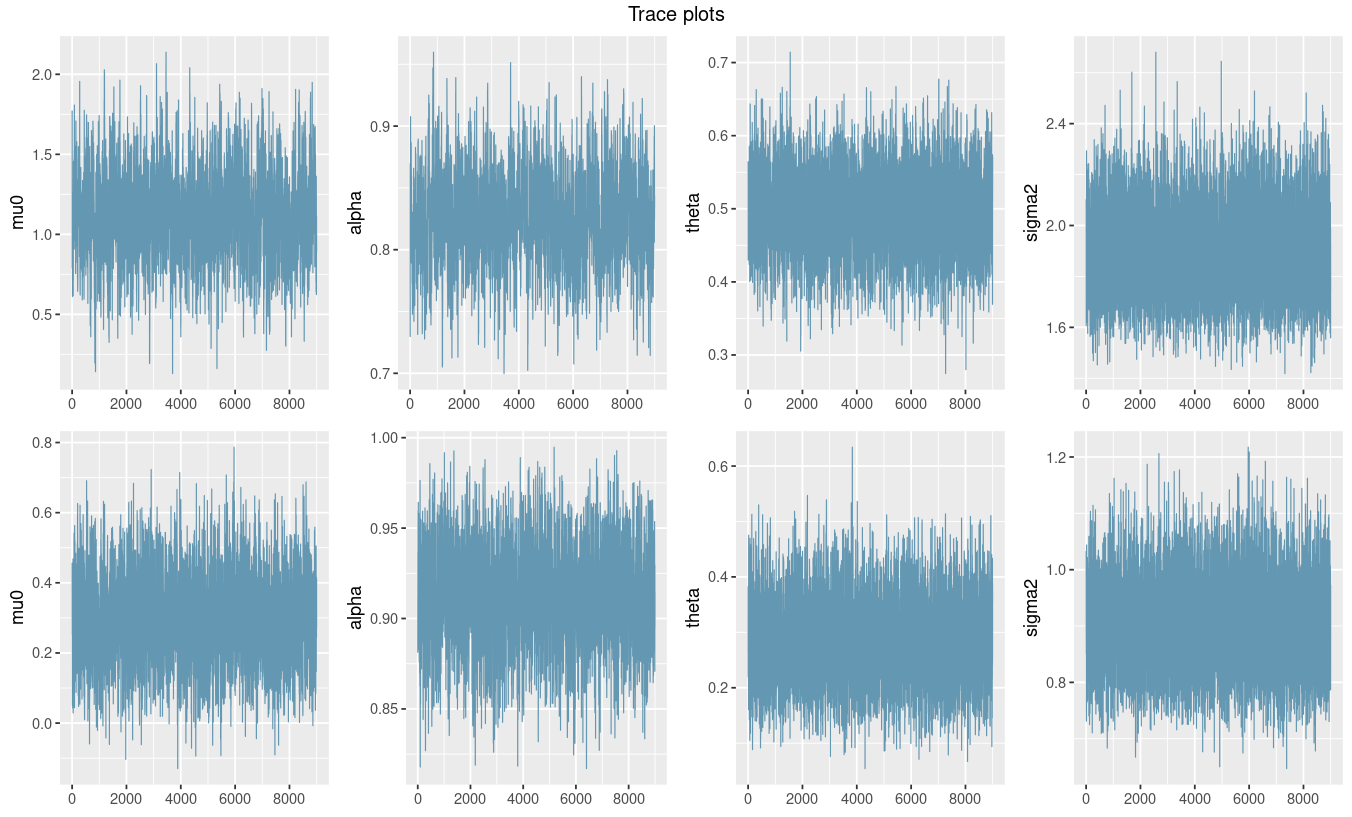
\includegraphics[width=0.9\textwidth]{images/4-ARMA/traceplots.png}
    \caption{Trace plots for the ARMA(1,1) models. The top line corresponds to the model used for GDP, while the bottom line corresponds to the model used for CPIAUCSL.}
\end{figure}
\begin{figure}[H]
    \centering
    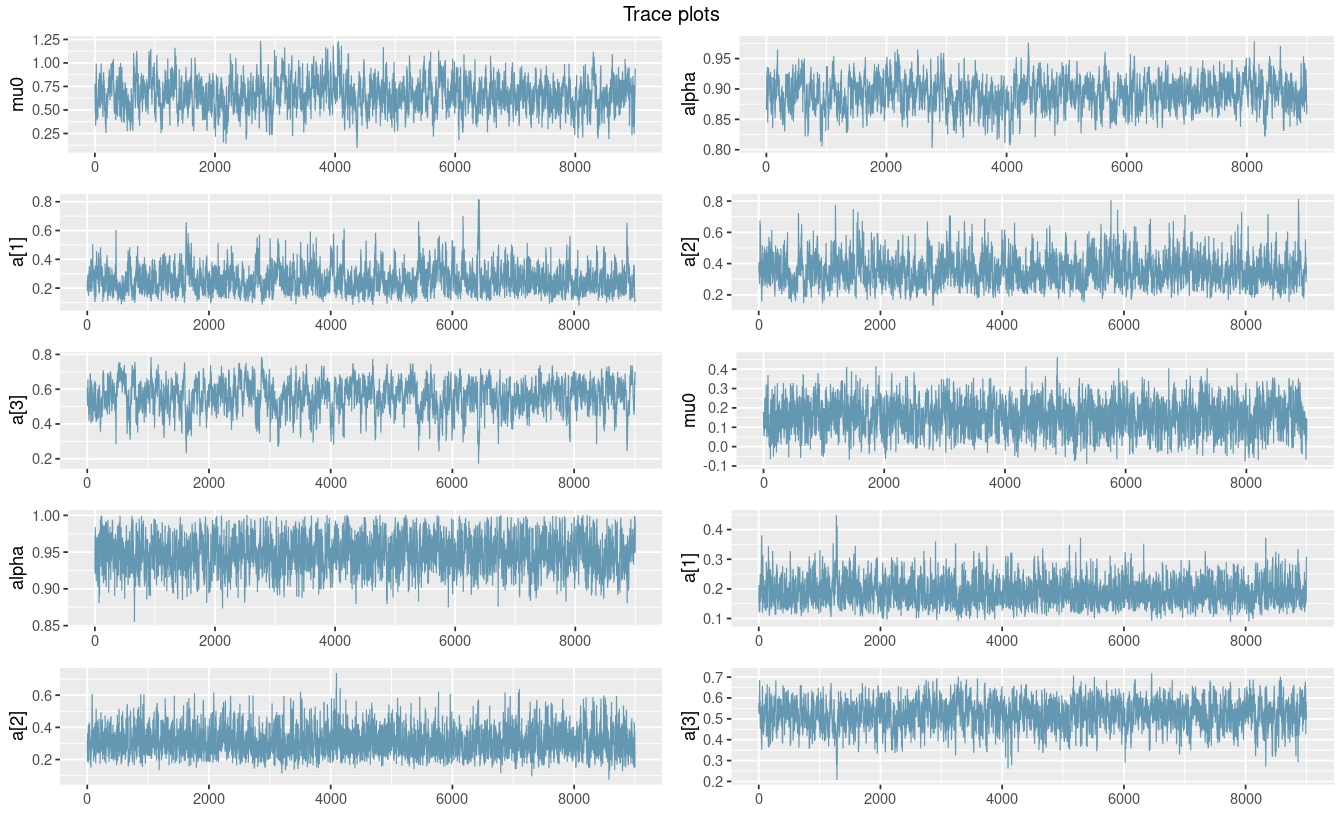
\includegraphics[width=0.9\textwidth]{images/5-GARCH/traceplots.png}
    \caption{Trace plots for the AR(1) + GARCH(1,1) models. The top line corresponds to the model used for GDP, while the bottom line corresponds to the model used for CPIAUCSL.}
\end{figure}
\begin{figure}[H]
    \centering
    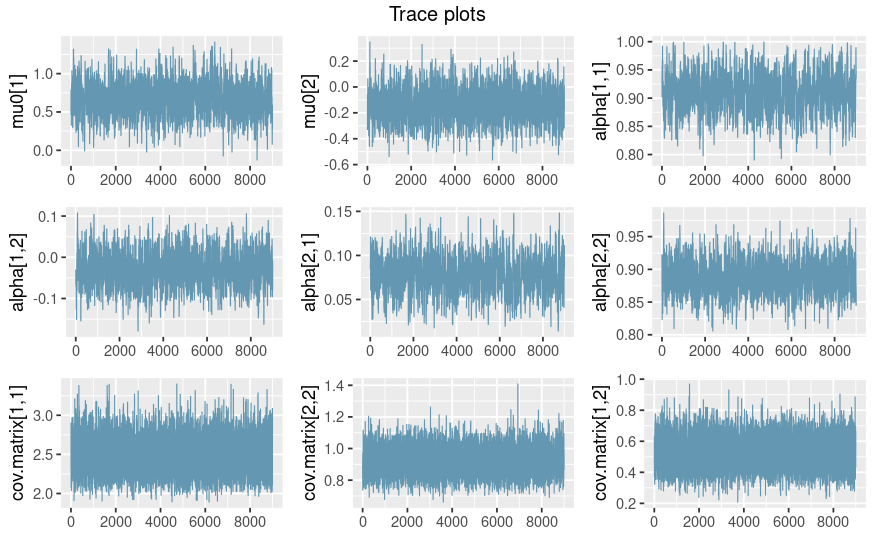
\includegraphics[width=0.9\textwidth]{images/6-VAR/traceplots.png}
    \caption{Trace plots for the VAR(1) model.}
\end{figure}
\subsection*{Comparison with public libraries}
In this section, we compared the in-sample predictions and the posterior distributions of our JAGS models with those obtained from public libraries. The comparison do not show significant differences, with the exception of MA and GARCH models where the posterior distributions of the parameters do not completely  match.
\begin{figure}[H]
    \centering
    \begin{minipage}{0.49\textwidth}
        \centering
        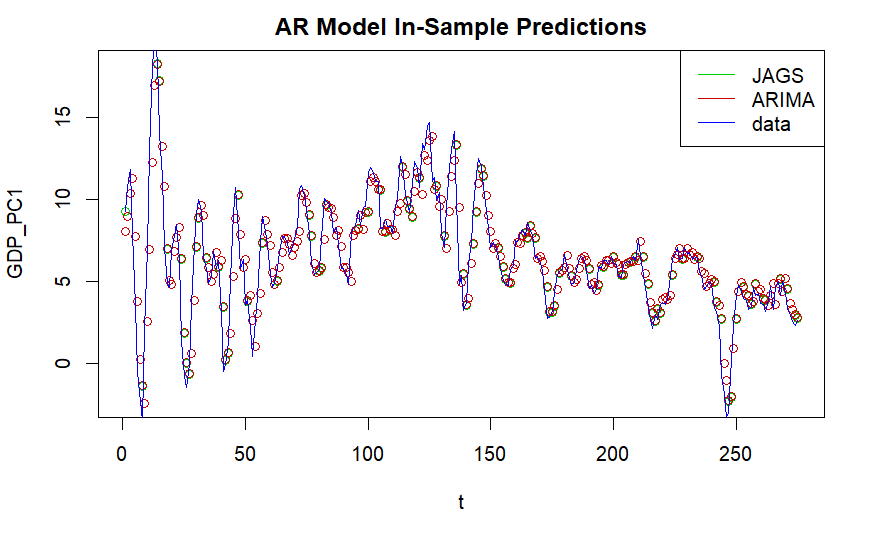
\includegraphics[width=\textwidth]{images/2-AR/ARIMA_predictions_gdp.png}
        \caption{In-sample predicions for GDP using AR(1) with JAGS and ARIMA.}
        \label{fig:ARIMA_AR_gdp_prediction}
    \end{minipage}\hfill
    \begin{minipage}{0.49\textwidth}
        \centering
        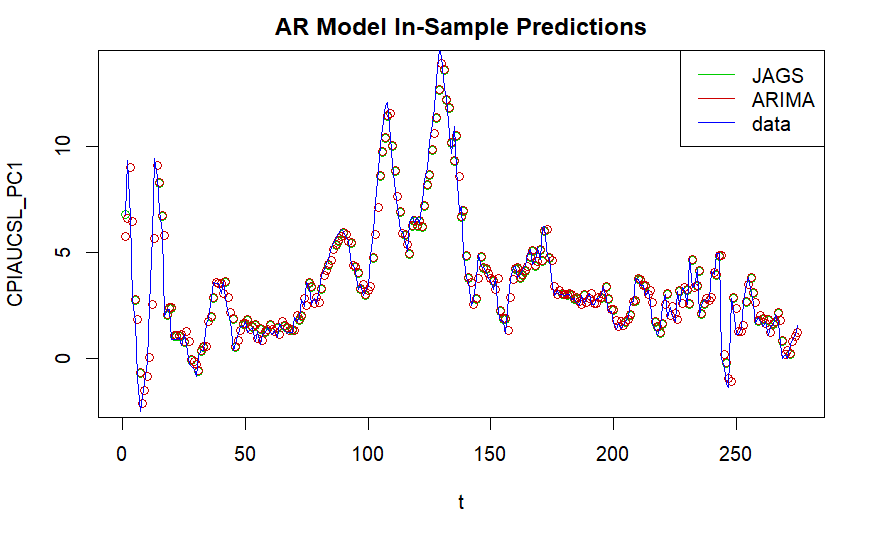
\includegraphics[width=\textwidth]{images/2-AR/ARIMA_predictions_infl.png}
        \caption{In-sample predicions for CPIAUCSL using AR(1) with JAGS and ARIMA.}
        \label{fig:ARIMA_AR_infl_prediction}
    \end{minipage}
\end{figure}
\begin{figure}[H]
    \centering
    \begin{minipage}{0.49\textwidth}
        \centering
        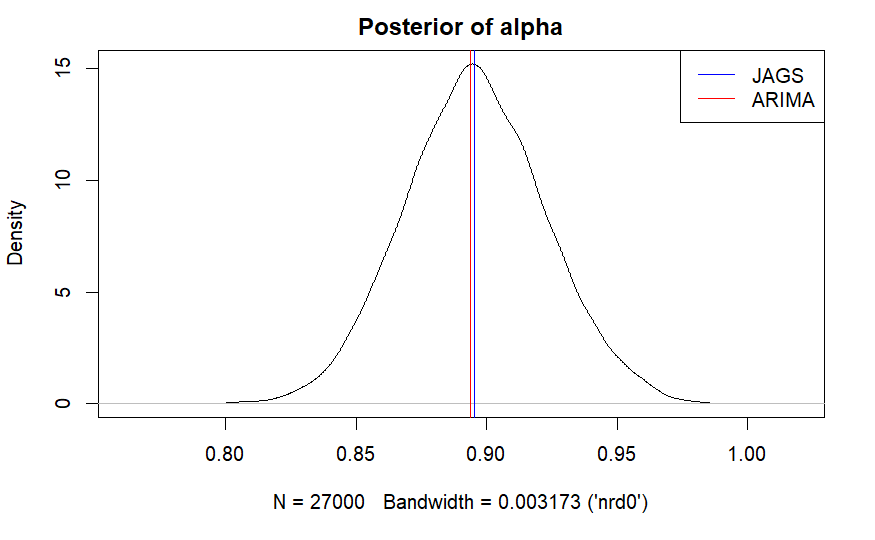
\includegraphics[width=\textwidth]{images/2-AR/ARIMA_posterior_distribution_gdp.png}
        \caption{Posterior distribution for the parameter of AR(1) compared with ARIMA estimated parameter for GDP.}
        \label{fig:ARIMA_AR_gdp_posteriors}
    \end{minipage}\hfill
    \begin{minipage}{0.49\textwidth}
        \centering
        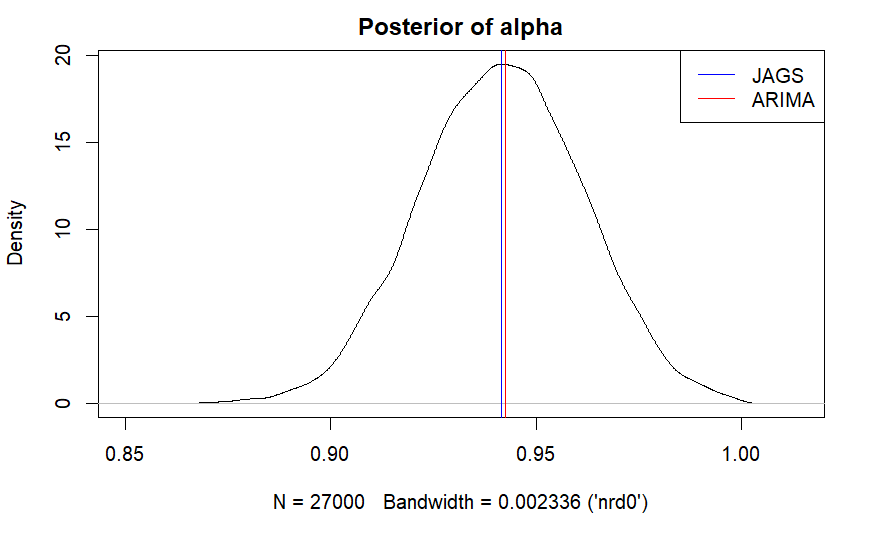
\includegraphics[width=\textwidth]{images/2-AR/ARIMA_posterior_distribution_infl.png}
        \caption{Posterior distribution for the parameter of AR(1) compared with ARIMA estimated parameter for CPIAUCSL.}
        \label{fig:ARIMA_AR_infl_posteriors}
    \end{minipage}
\end{figure}
\begin{figure}[H]
    \centering
    \begin{minipage}{0.49\textwidth}
        \centering
        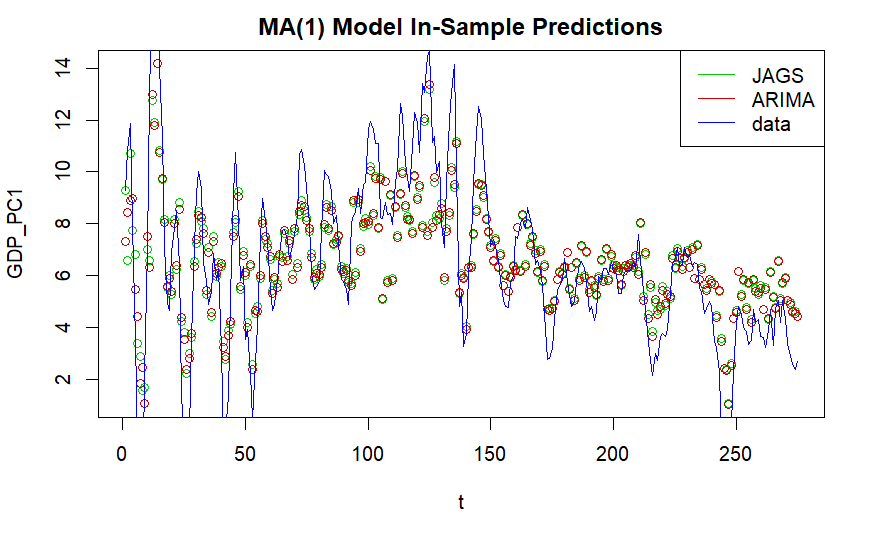
\includegraphics[width=\textwidth]{images/3-MA/ARIMA_MA1_predictions_gdp.png}
        \caption{In-sample predicions for GDP using MA(1) with JAGS and ARIMA.}
        \label{fig:ARIMA_MA1_gdp_prediction}
    \end{minipage}\hfill
    \begin{minipage}{0.49\textwidth}
        \centering
        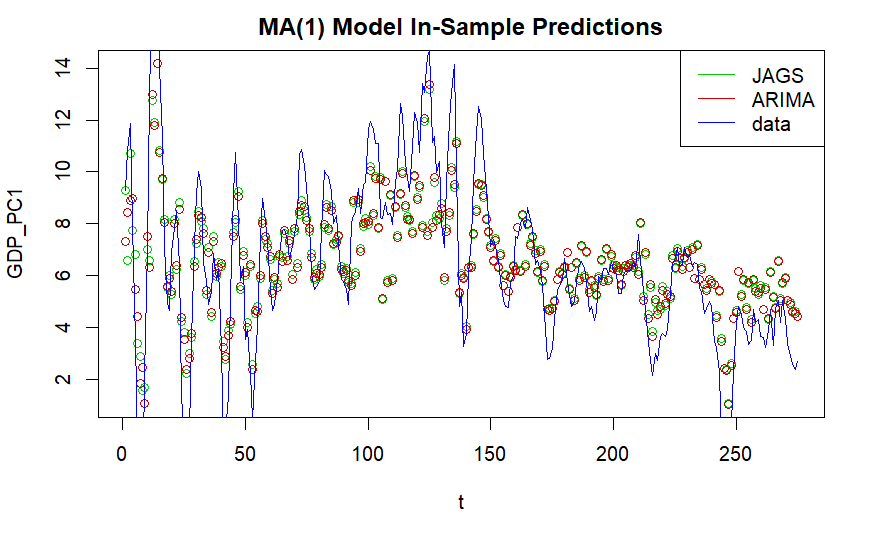
\includegraphics[width=\textwidth]{images/3-MA/ARIMA_MA1_predictions_gdp.png}
        \caption{In-sample predicions for CPIAUCSL using MA(1) with JAGS and ARIMA.}
        \label{fig:ARIMA_MA1_infl_prediction}
    \end{minipage}
\end{figure}
\begin{figure}[H]
    \centering
    \begin{minipage}{0.49\textwidth}
        \centering
        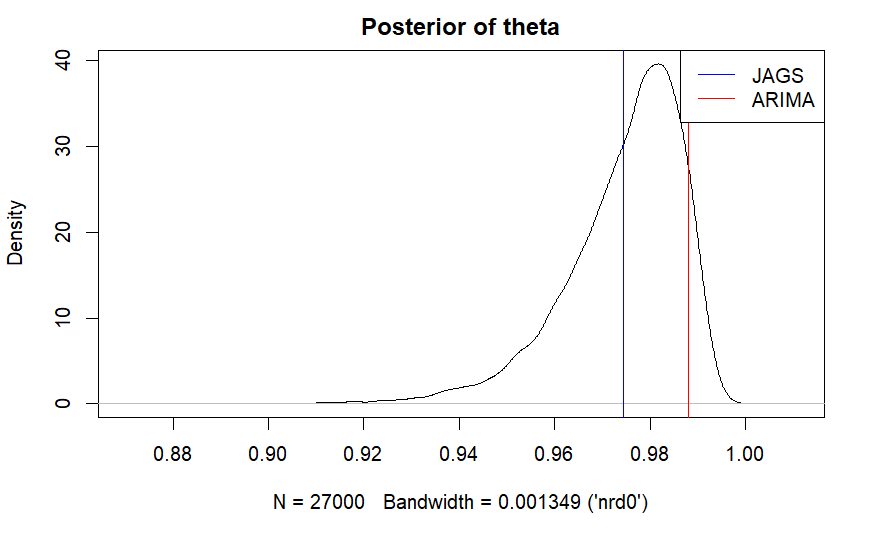
\includegraphics[width=\textwidth]{images/3-MA/ARIMA_MA1_posterior_distribution_gdp.png}
        \caption{Posterior distribution for the parameter of MA(1) compared with ARIMA estimated parameter for GDP.}
        \label{fig:ARIMA_MA1_gdp_posteriors}
    \end{minipage}\hfill
    \begin{minipage}{0.49\textwidth}
        \centering
        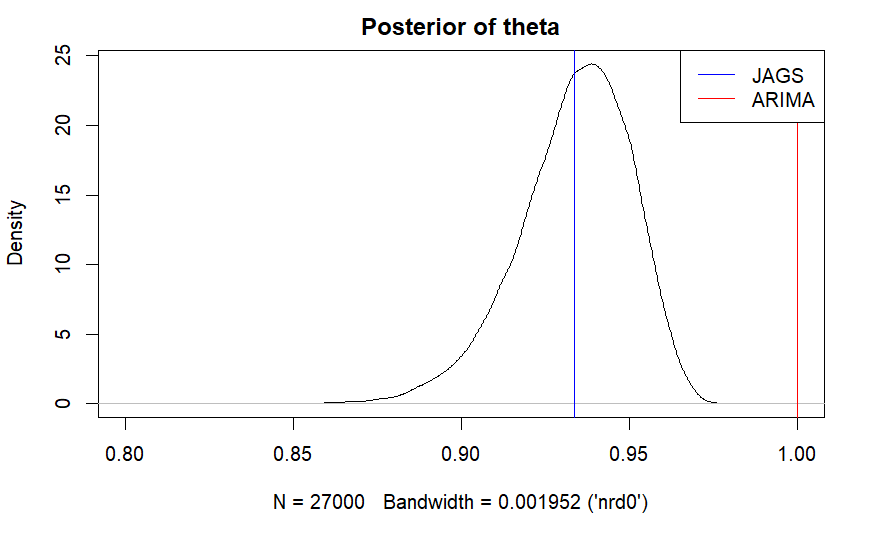
\includegraphics[width=\textwidth]{images/3-MA/ARIMA_MA1_posterior_distribution_infl.png}
        \caption{Posterior distribution for the parameter of MA(1) compared with ARIMA estimated parameter for CPIAUCSL.}
        \label{fig:ARIMA_MA1_infl_posteriors}
    \end{minipage}
\end{figure}
\begin{figure}[H]
    \centering
    \begin{minipage}{0.49\textwidth}
        \centering
        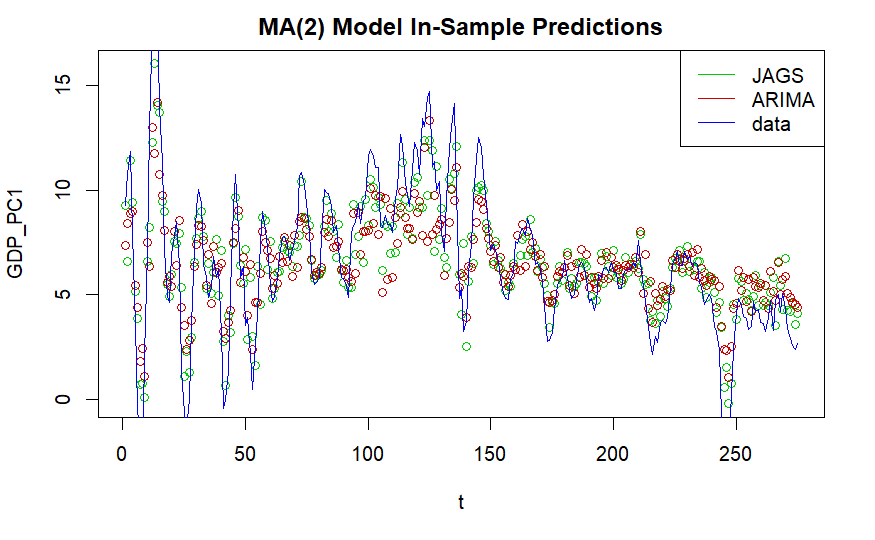
\includegraphics[width=\textwidth]{images/3-MA/ARIMA_MA2_predictions_gdp.png}
        \caption{In-sample predicions for GDP using MA(2) with JAGS and ARIMA.}
        \label{fig:ARIMA_MA2_gdp_prediction}
    \end{minipage}\hfill
    \begin{minipage}{0.49\textwidth}
        \centering
        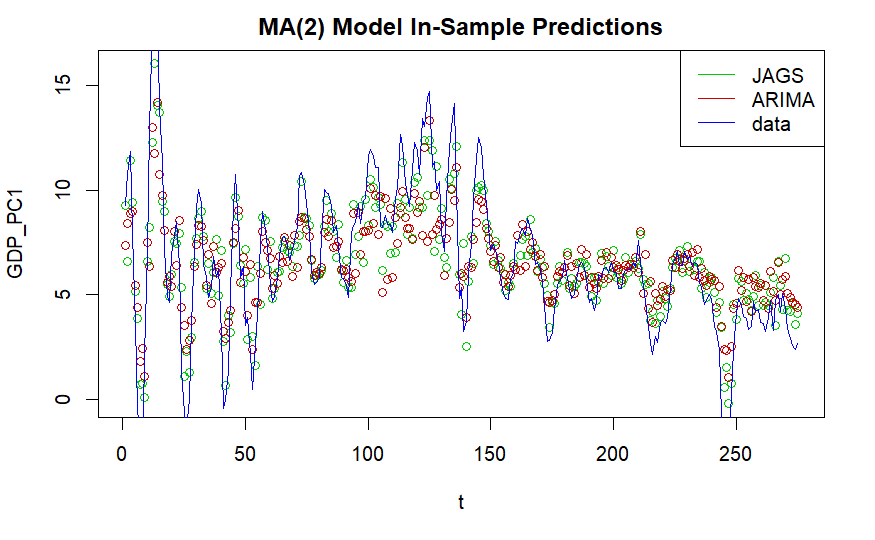
\includegraphics[width=\textwidth]{images/3-MA/ARIMA_MA2_predictions_gdp.png}
        \caption{In-sample predicions for CPIAUCSL using MA(2) with JAGS and ARIMA.}
        \label{fig:ARIMA_MA2_infl_prediction}
    \end{minipage}
\end{figure}
\begin{figure}[H]
    \centering
    \begin{minipage}{0.49\textwidth}
        \centering
        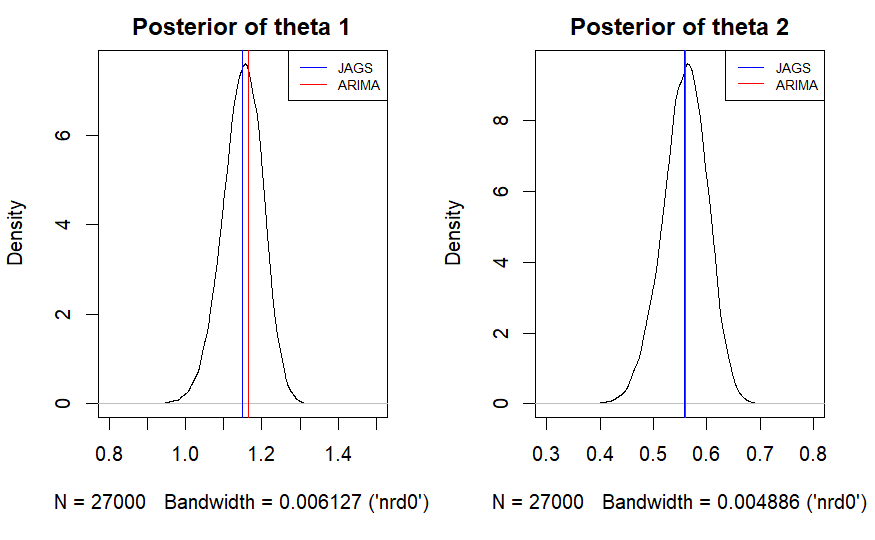
\includegraphics[width=\textwidth]{images/3-MA/ARIMA_MA2_posterior_distribution_gdp.png}
        \caption{Posterior distribution for the parameters of MA(2) compared with ARIMA estimated parameters for GDP.}
        \label{fig:ARIMA_MA2_gdp_posteriors}
    \end{minipage}\hfill
    \begin{minipage}{0.49\textwidth}
        \centering
        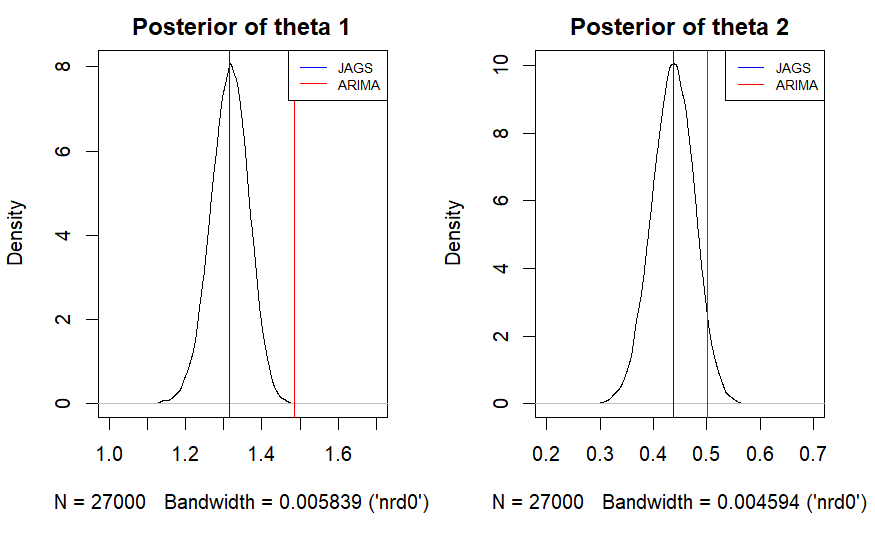
\includegraphics[width=\textwidth]{images/3-MA/ARIMA_MA2_posterior_distribution_infl.png}
        \caption{Posterior distribution for the parameters of MA(2) compared with ARIMA estimated parameters for CPIAUCSL.}
        \label{fig:ARIMA_MA2_infl_posteriors}
    \end{minipage}
\end{figure}
\begin{figure}[H]
    \centering
    \begin{minipage}{0.49\textwidth}
        \centering
        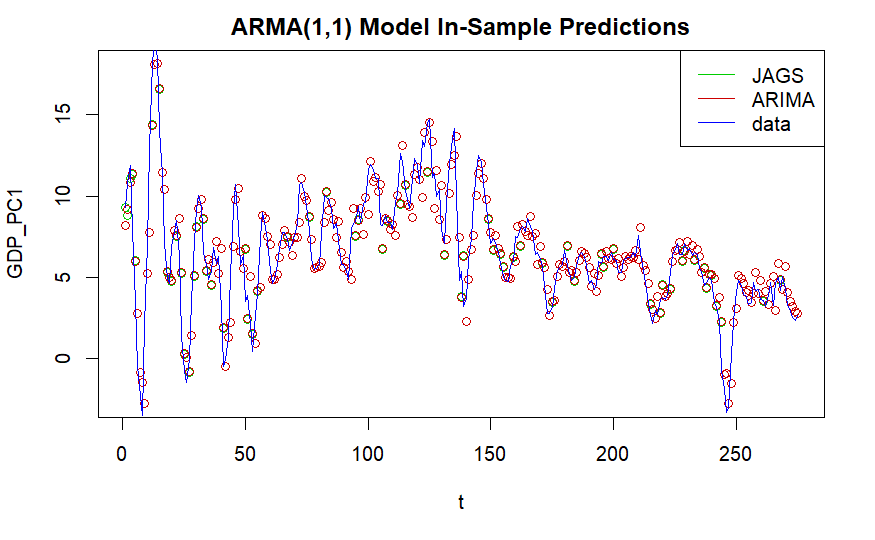
\includegraphics[width=\textwidth]{images/4-ARMA/ARIMA_ARMA_predictions_gdp.png}
        \caption{In-sample predicions for GDP using ARMA(1,1) with JAGS and ARIMA.}
        \label{fig:ARIMA_ARMA_gdp_prediction}
    \end{minipage}\hfill
    \begin{minipage}{0.49\textwidth}
        \centering
        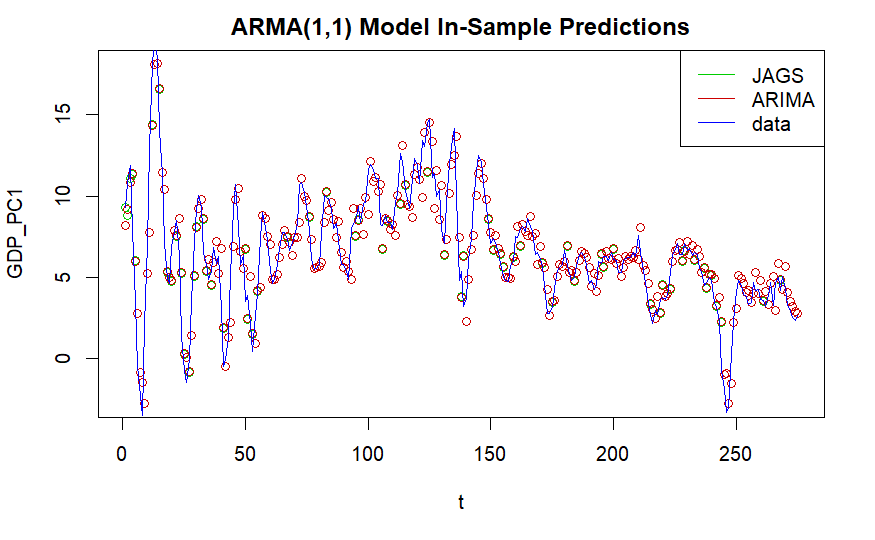
\includegraphics[width=\textwidth]{images/4-ARMA/ARIMA_ARMA_predictions_gdp.png}
        \caption{In-sample predicions for CPIAUCSL using ARMA(1,1) with JAGS and ARIMA.}
        \label{fig:ARIMA_ARMA_infl_prediction}
    \end{minipage}
\end{figure}
\begin{figure}[H]
    \centering
    \begin{minipage}{0.49\textwidth}
        \centering
        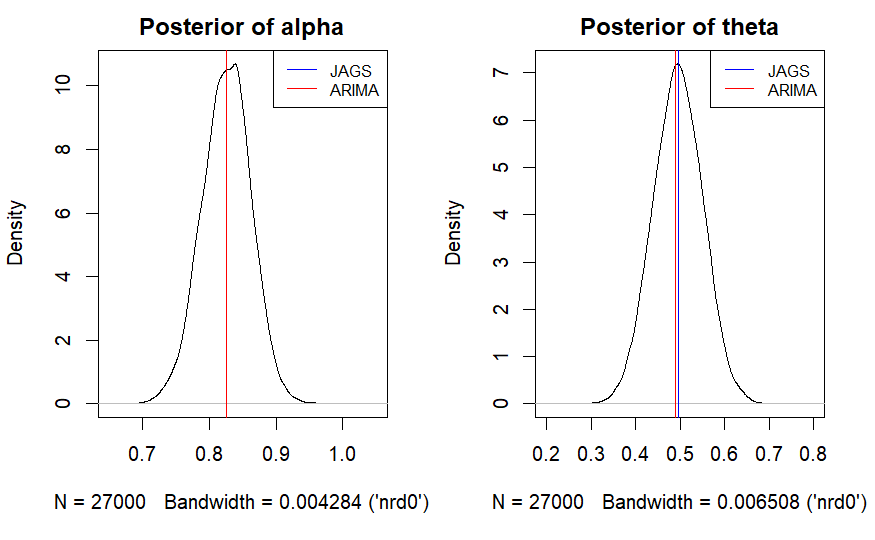
\includegraphics[width=\textwidth]{images/4-ARMA/ARIMA_ARMA_posterior_distribution_gdp.png}
        \caption{Posterior distribution for the parameters of ARMA(1,1) compared with ARIMA estimated parameters for GDP.}
        \label{fig:ARIMA_ARMA_gdp_posteriors}
    \end{minipage}\hfill
    \begin{minipage}{0.49\textwidth}
        \centering
        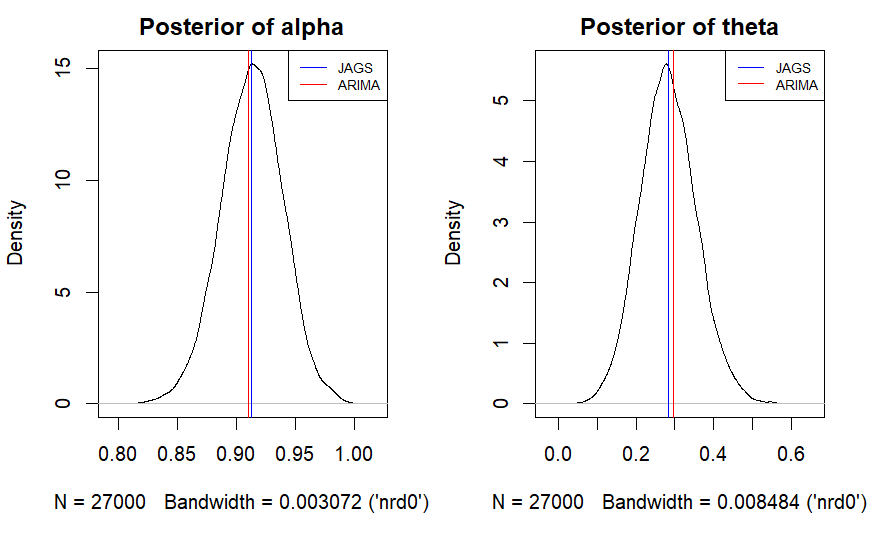
\includegraphics[width=\textwidth]{images/4-ARMA/ARIMA_ARMA_posterior_distribution_infl.png}
        \caption{Posterior distribution for the parameters of ARMA(1,1) compared with ARIMA estimated parameters for CPIAUCSL.}
        \label{fig:ARIMA_ARMA_infl_posteriors}
    \end{minipage}
\end{figure}
\begin{figure}[H]
    \centering
    \begin{minipage}{0.49\textwidth}
        \centering
        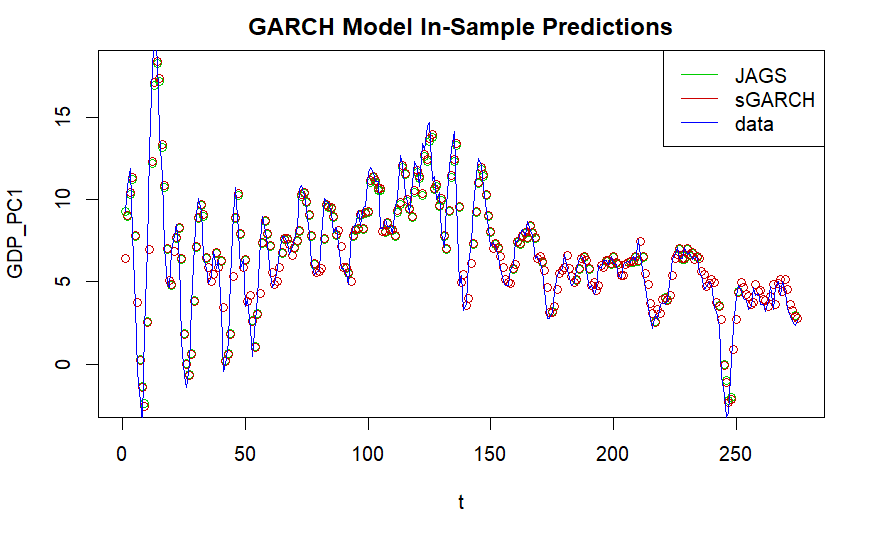
\includegraphics[width=\textwidth]{images/5-GARCH/GARCH_predictions_gdp.png}
        \caption{In-sample predicions for GDP using GARCH(1,1) + AR(1) with JAGS and uGarch.}
        \label{fig:GARCH_gdp_prediction}
    \end{minipage}\hfill
    \begin{minipage}{0.49\textwidth}
        \centering
        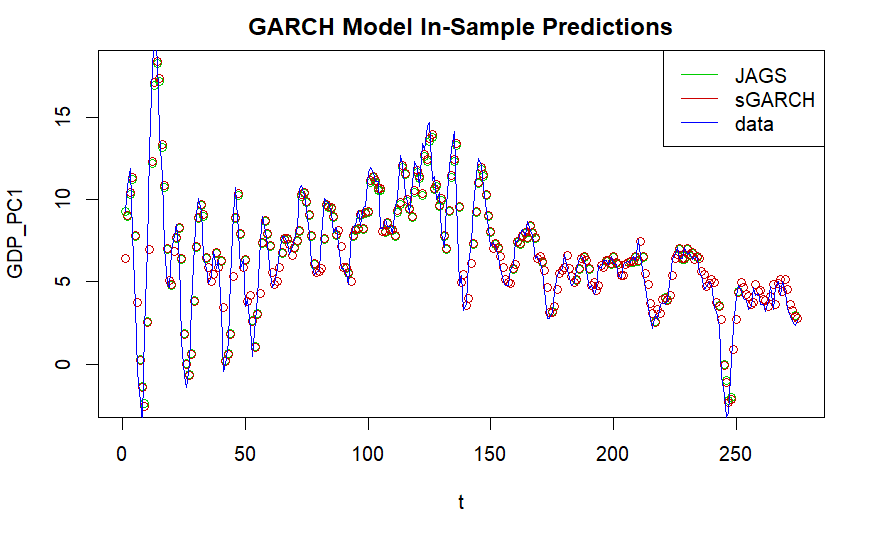
\includegraphics[width=\textwidth]{images/5-GARCH/GARCH_predictions_gdp.png}
        \caption{In-sample predicions for CPIAUCSL using GARCH(1,1) + AR(1) with JAGS and uGarch.}
        \label{fig:GARCH_infl_prediction}
    \end{minipage}
\end{figure}
\begin{figure}[H]
    \centering
    \begin{minipage}{0.49\textwidth}
        \centering
        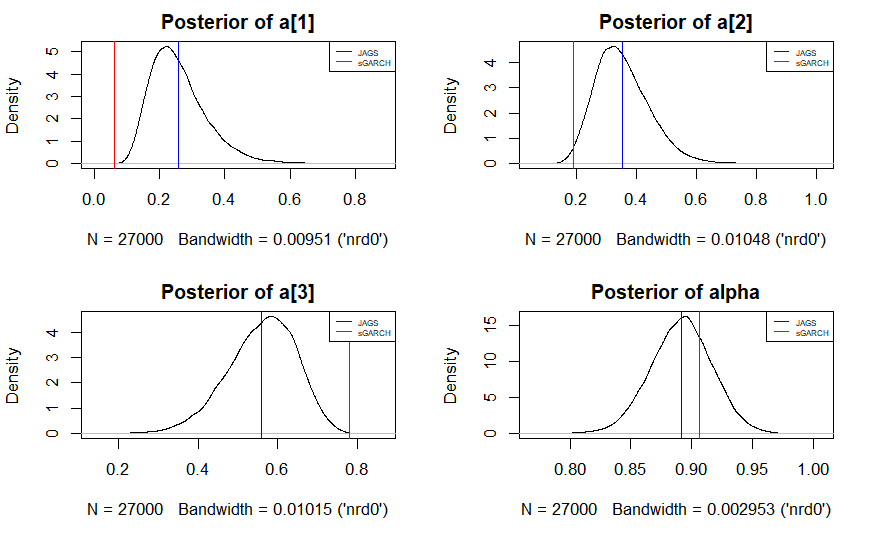
\includegraphics[width=\textwidth]{images/5-GARCH/GARCH_posterior_distribution_gdp.png}
        \caption{Posterior distribution for the parameters of GARCH(1,1) + AR(1) compared with uGarch estimated parameters for GDP.}
        \label{fig:GARCH_gdp_posteriors}
    \end{minipage}\hfill
    \begin{minipage}{0.49\textwidth}
        \centering
        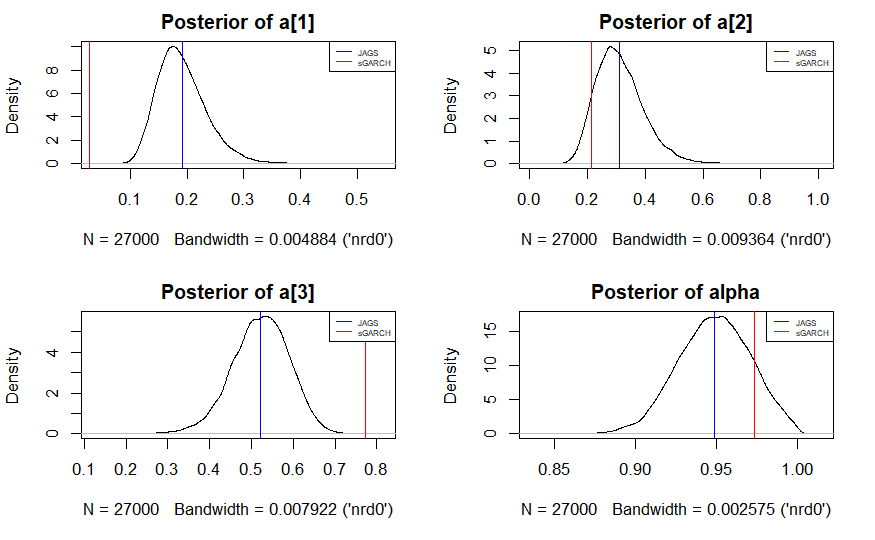
\includegraphics[width=\textwidth]{images/5-GARCH/GARCH_posterior_distribution_infl.png}
        \caption{Posterior distribution for the parameters of GARCH(1,1) + AR(1) compared with uGarch estimated parameters for CPIAUCSL.}
        \label{fig:GARCH_infl_posteriors}
    \end{minipage}
\end{figure}
\begin{figure}[H]
    \centering
    \begin{minipage}{0.49\textwidth}
        \centering
        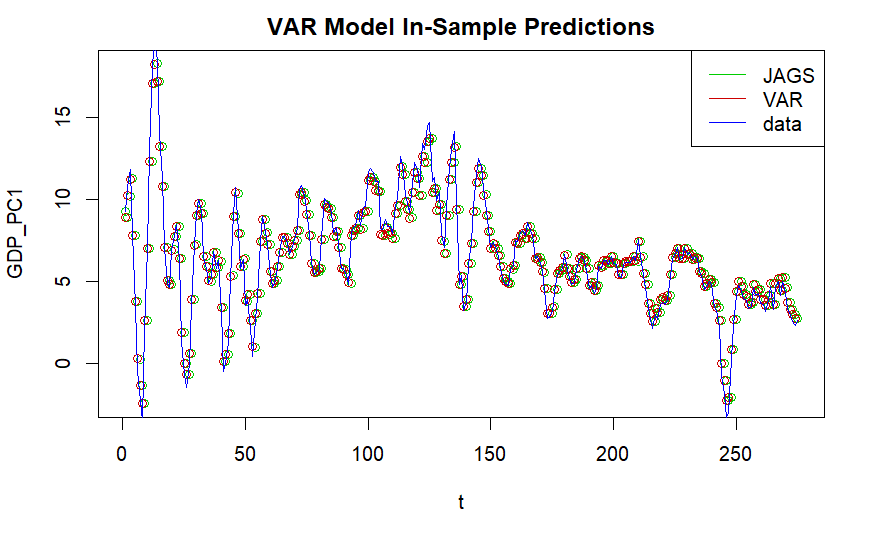
\includegraphics[width=\textwidth]{images/6-VAR/VAR_predictions_gdp.png}
        \caption{In-sample predicions for GDP using VAR(1) with JAGS and VAR.}
        \label{fig:VAR_gdp_prediction}
    \end{minipage}\hfill
    \begin{minipage}{0.49\textwidth}
        \centering
        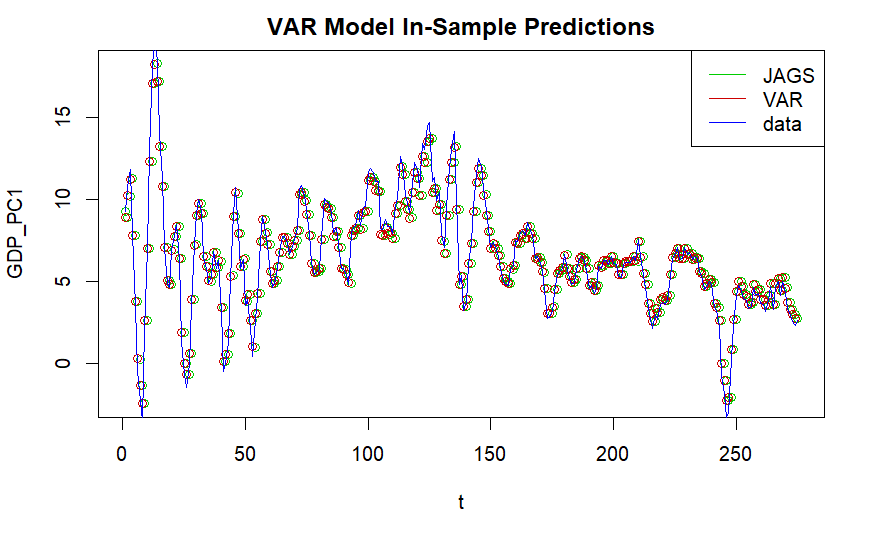
\includegraphics[width=\textwidth]{images/6-VAR/VAR_predictions_gdp.png}
        \caption{In-sample predicions for CPIAUCSL using VAR(1) with JAGS and VAR.}
        \label{fig:VAR_infl_prediction}
    \end{minipage}
\end{figure}
\begin{figure}[H]
    \centering
    \begin{minipage}{0.49\textwidth}
        \centering
        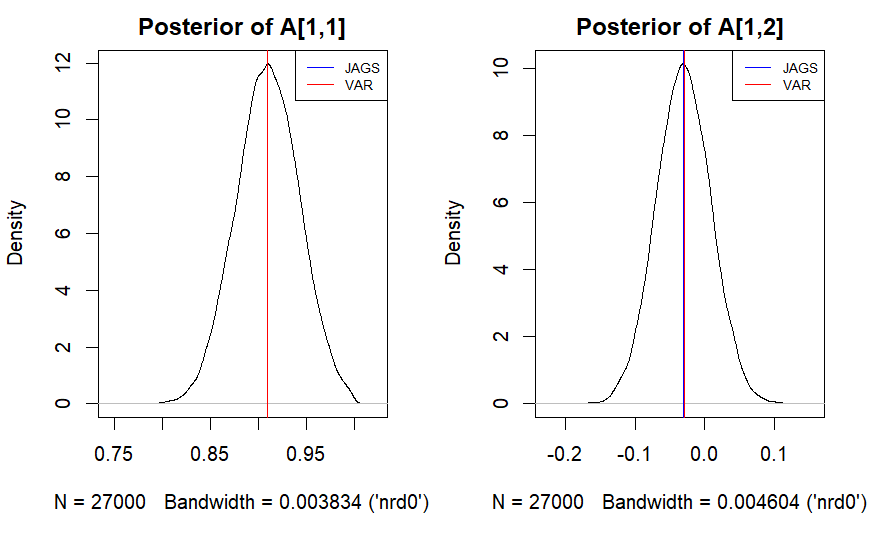
\includegraphics[width=\textwidth]{images/6-VAR/VAR_posterior_distribution_gdp.png}
        \caption{Posterior distribution for the parameters of VAR(1) compared with VAR estimated parameters for GDP.}
        \label{fig:VAR_gdp_posteriors}
    \end{minipage}\hfill
    \begin{minipage}{0.49\textwidth}
        \centering
        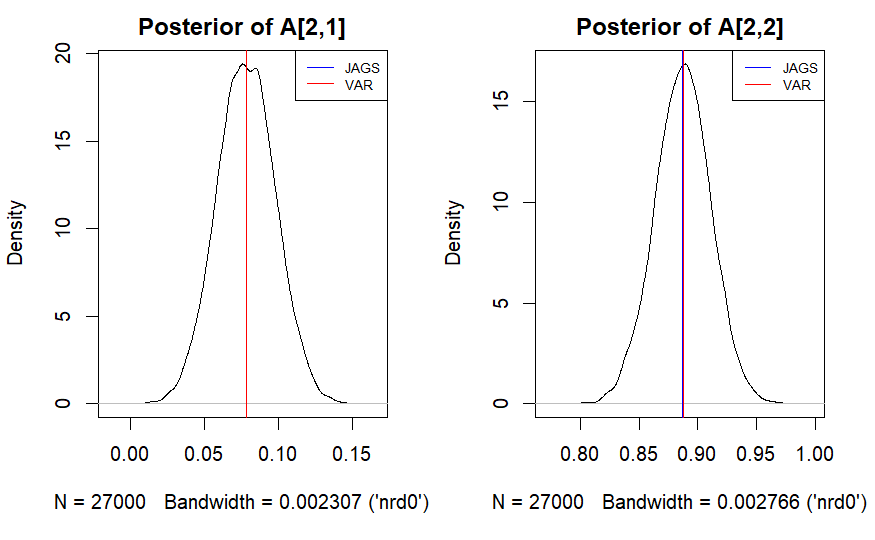
\includegraphics[width=\textwidth]{images/6-VAR/VAR_posterior_distribution_infl.png}
        \caption{Posterior distribution for the parameters of VAR(1) compared with VAR estimated parameters for CPIAUCSL.}
        \label{fig:VAR_infl_posteriors}
    \end{minipage}
\end{figure}